\documentclass{protokol}

\usepackage[czech]{babel}
\usepackage[utf8]{inputenc}
\usepackage{icomma}

% Plovouci bloky (obrazky, tabulky)
\usepackage{floatrow}
\floatsetup[table]{capposition=top}
\floatsetup[figure]{frameset={\fboxsep16pt}}
\usepackage{subcaption}

% Tabulky
\usepackage{tabu}
\usepackage{booktabs}
\usepackage{csvsimple}
\usepackage{multirow}
\usepackage{multicol}
\usepackage{pgfplotstable}
\pgfplotsset{compat=1.17}
\pgfplotstableset{
	use comma,
	set thousands separator = {},
}

% Jednotky
\usepackage{siunitx}
\sisetup{
	locale               = DE,
	inter-unit-product   = \ensuremath{{}\cdot{}},
	list-units           = single,
	list-separator       = {; },
	list-final-separator = \text{ a },
	list-pair-separator  = \text{ a },
	range-phrase         = \text{ až },
	range-units          = single,
}
\usepackage{amsmath}

% Obvody
\usepackage{circuitikz}

% Obrazky a grafy
% \usepackage{graphicx}
\graphicspath{
	{img/}
	{plots/}
	{build/plots/}
}
\usepackage{epstopdf}
\epstopdfsetup{outdir=./build/plots/}

\usepackage[hidelinks,pdfusetitle]{hyperref}
\usepackage[backend=biber, sorting=none, sortlocale=cs_CZ]{biblatex}
\addbibresource{references.bib}

\title{Langmuirova sonda}
\author{Pavel Kosík, Jan Slaný}

\jmenopraktika={Praktikum z fyziky plazmatu}  % jmeno predmetu
\jmeno={Pavel Kosík, Jan Slaný}                             % jmeno mericiho
\obor={F}                               % zkratka studovaneho oboru
\skupina={Út 15:00}                     % doba vyuky seminarni skupiny
\rocnik={IV}
\semestr={VIII}

\cisloulohy={03}
\jmenoulohy={Langmuirova sonda}

\datum={8. března 2022}                  % datum mereni ulohy
\tlak={}% [hPa]
\teplota={}% [C]
\vlhkost={}% [%]

\newcommand\elemcharge{e}
\newcommand\boltzmann{k}
% \newcommand\boltzmann{k_\mathrm{B}}
\newcommand\masselec{m_\mathrm{e}}
\newcommand{\tgh}{\mathrm{tgh}}

\newcommand\pres{p}
\newcommand\idisch{I_\mathrm{d}}
\newcommand\iprobe{I_\mathrm{s}}
\newcommand\iion{I_\mathrm{i}}
\newcommand\ielec{I_\mathrm{e}}
\newcommand\flpot{V_\mathrm{fl}}
\newcommand\plpot{V_\mathrm{p}}
\newcommand\plpota{V_\mathrm{p,a}}
\newcommand\plpotd{V_\mathrm{p,d}}
\newcommand\potprobe{V_\mathrm{s}}
\newcommand\uprobe{U_\mathrm{s}}
\newcommand\didu{\frac{\mathrm d^2 \ielec}{\mathrm d \uprobe^2}}
\newcommand\dension{n_\mathrm{i}}
\newcommand\denselec{n_\mathrm{e}}
\newcommand\enelec{\mathcal E_\mathrm{e}}
\newcommand\eedf{f(\enelec)}
\newcommand\ueedf{\varepsilon}
\newcommand\probesurf{S}
\newcommand\sheathsurf{S_\mathrm{s}}
\newcommand\tempion{T_\mathrm{i}}
\newcommand\tempelec{T_\mathrm{e}}
\newcommand\tempeleca{T_\mathrm{e,a}}
\newcommand\tempelecp{T_\mathrm{e,p}}
\newcommand\tempelecf{T_\mathrm{e,f}}
\newcommand\massion{M}
\newcommand\tim{t}

\newcommand\iioni{I_{\mathrm{i}1}}
\newcommand\iionii{I_{\mathrm{i}2}}
\newcommand\iionsat{I_{\mathrm{i}0}}
\newcommand\ieleci{I_{\mathrm{e}1}}
\newcommand\ielecii{I_{\mathrm{e}2}}
\newcommand\idouble{I_{\mathrm{c}}}
\newcommand\poti{V_1}
\newcommand\potii{V_2}
\newcommand\udouble{U_\mathrm{d}}
\newcommand\udoubleprobe{\udouble}
\newcommand\denseleca{n_\mathrm{e,a}}
\newcommand\denselecf{n_\mathrm{e,f}}
\newcommand\denselecfii{n_{\mathrm{e,f}2}}
\newcommand\speedion{v_\mathrm{i}}
\newcommand\speedelec{v_\mathrm{e}}
\newcommand\eqresist{R_0}

\begin{document}
\header

\section{Úvod}
\label{sec:intro}
\newcommand\parta{A}
\newcommand\partb{B}
\newcommand\partc{C}
\newcommand\slopeb{\beta}
Předmětem této úlohy je studium kladného sloupce doutnavého výboje
pomocí Langmuirovy sondy.
Tato metoda umožňuje stanovit důležité parametry plazmatu jako je
elektronová hustota, rozdělovací funkce rychlostí elektronů
a s~ní spojená teplota elektronů.

Langmuirovou sondou rozumíme malý vodič zavedený do~plazmatu.
Při změně elektrického napětí mezi sondou a~plazmatem je možno pozorovat
změnu proudu, který jí protéká.
Tato závislost je takzvaná voltampérová charakteristika sondy
a~její analýza umožňuje určit zmíněné parametry.
Přítomnost sondy však zkoumané plazma ovlivňuje,
pročež je vhodné, aby její rozměry byly co nejmenší.

Označme potenciál neporušeného plazmatu~$\plpot$,
potenciál sondy~$\potprobe$ a~proud protékající sondou~$\iprobe$.
Potenciál se obvykle určuje vzhledem k~referenční elekrodě,
ale při popisu chování sondy je vhodnější jej vztáhnout k~plazmovému
potenciálu.
Definujme proto napětí sondy $\uprobe$ jako:
\begin{equation}
	\label{eq:uprobe}
	\uprobe = \potprobe - \plpot.
\end{equation}

Podle počtu součástí je možno rozlišit několik druhů sond,
tato úloha se zaměřuje na dva nejjednodušší: jednoduchou a~dvojnou sondu.

\subsection{Jednoduchá sonda}
\label{sec:intro-simple}
Jednoduchá Langmuirova sonda sestává z~jediného vodiče vnořeného do plazmatu.
Typická voltampérová chrakteristika rovinné sondy je na~obrázku
č.~\ref{fig:vac-simple} a~její průběh můžeme rozdělit na tři oblasti.

\begin{figure}[hbp]
	\centering
	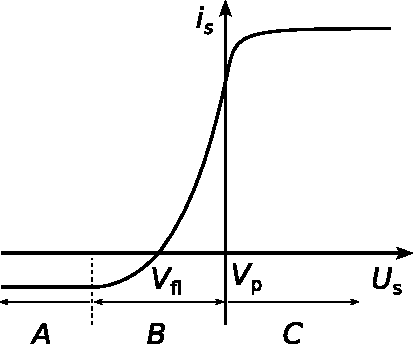
\includegraphics{vac-simple}
	\caption{Voltampérová charakteristika jednoduché sondy.
		Převzato z~\autocite{assignment-simpleprobe}.}
	\label{fig:vac-simple}
\end{figure}

\subsubsection{Oblast saturovaného proudu \parta}
Pokud je sonda výrazně záporně nabitá vzhledem k potenciálu plazmatu,
uplatní se Debyeovo stínění a~v~okolí sondy vznikne vrstva kladného
prostorového náboje.
Jelikož v této vrstvě nejsou elektrony, nemůže zde probíhat rekombinace,
ionizace, ani excitace nárazem elektronu a kolem sondy pozorujeme temný prostor.
Proud dopadající na sondu je převážně iontový
a~jeho velikost se řídí Child-Langmuirovým zákonem.

\subsubsection{Přechodová oblast \partb}
Při zvýšení napětí na sondě získají některé elektrony dostatečnou energii na to,
aby překonaly stěnovou vrstvu a dopadly na povrch sondy.
Iontový proud stále převládá.
Absolutní hodnota proudu s~rostoucím napětím na sondě klesá.
Bod, pro nějž je roven nule (tedy tam, kde se proudové příspěvky vyrovnají)
se nazývá plovoucí potenciál $\flpot$.
Další zvyšování napětí na sondě $\potprobe$ má za následek růst celkového proudu.
Zde již převládá proud elektronový $\ielec$, jehož průběh v~této oblasti lze
za předpokladu Maxwell-Boltzmannova rozdělení popsat vztahem:
\begin{equation}
	\label{eq:partb}
	\ielec = \probesurf \elemcharge \denselec
		\sqrt{\frac{\boltzmann \tempelec}{2 \pi \masselec}}
		e^{\frac{-\elemcharge\uprobe}{\boltzmann \tempelec}},
\end{equation}
kde $\probesurf$ je plocha sondy, $\denselec$ koncentrace elektronů,
$\boltzmann$ Boltzmanova konstanta, $\tempelec$ elektronová teplota,
$\elemcharge$~elementární náboj a~$\masselec$ hmotnost elektronu.
Nastává změna polarizace sondy.
Ze~vztahu \eqref{eq:partb} plyne,
že závislost $\ln(\ielec)=f(\uprobe)$ by měla být lineární.
Směrnice přímky potom určuje teplotu elektronů $\tempelec$
a~konstantní člen koncentraci elektronů $\denselec$.

\subsubsection{Oblast saturovaného elektronového proudu \partc}
Je-li překročeno nulové napětí $\uprobe$ na sondě
(tedy je-li sonda nabita vzhledem k potenciálu plazmatu $\plpot$ kladně),
začíná sonda přitahovat elektrony a odpuzovat kladné ionty.

V~případě válcové sondy proud v~této oblasti parabolicky roste.

\subsection{Dvojná sonda}
Dvojnou sondou rozumíme dvě shodné Langmuirovy sondy vnořené do plazmatu;
jejich plochy $\probesurf_1$ a~$\probesurf_2$ považujeme za shodné.
Vzájemná vzdálenost sond musí být taková, aby se jejich stěnové vrstvy
nepřekrývaly.
Schéma dvojné sondy je znázorněno na obrázku č.~\ref{fig:probe-double}.
Iontové proudy jednotlivých sond jsou označeny $\iioni$ a $\iionii$,
elektronové proudy $\ieleci$ a $\ielecii$.
Veličina $\idouble$ značí proud tekoucí mezi sondami,
takzvaný cirkulační proud.

\begin{figure}[hbp]
	\centering
	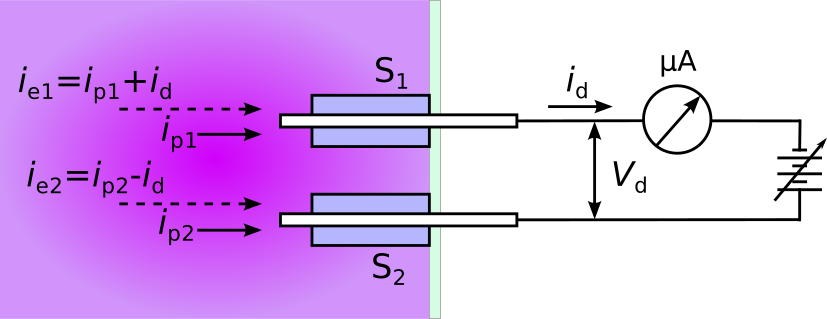
\includegraphics{probe-double}
	\caption{Schéma dvojné sondy.
		Převzato z~\autocite{assignment-doubleprobe}.}
	\label{fig:probe-double}
\end{figure}

Voltampérová charakteristika dvojné sondy je závislost cirkulačního proudu
na napětí $\udouble = \potii - \poti$ mezi sondami.
Příklad takové charakteristiky je znázorněn na obrázku č.~\ref{fig:vac-double}.
Pokud je napětí $\udouble$ nulové, tečou na obě sondy stejné proudy.
Při snižování $\udouble$ do záporných hodnot se potenciál první sondy $\poti$
blíží potenciálu plazmatu a roste proud $\ieleci$,
proud $\ielecii$ naopak klesá.
Další snižování $\udouble$ vede až k~tomu,
že proud $\ielecii$ vymizí a~veškeré elektrony dopadají na první sondu.
V~ideálním případě je proud $\idouble$ dále konstantní,
což odpovídá nasycenému iontovému proudu $\iionii$.
Při skutečném měření proud $\idouble$ dále mírně poroste.
Kladná napětí $\udouble$ vykazují stejné chování v~důsledku symetrie soustavy.

Voltampérovou charakteristiku ideální dvojné sondy lze aproximovat
následujícím vztahem:
\begin{equation}
	\label{eq:double-ideal}
	\idouble = \iionsat \, \tgh \left(
		\frac{\elemcharge\udouble}{\boltzmann\tempelec} \right).
\end{equation}
Zde $\tempelec$ je elektronová teplota
a~$\iionsat$ je saturovaný iontový proud, jehož velikost lze přibližně
vyjádřit jako:
\begin{equation}
	\label{eq:double-iionsat}
	\iionsat = \num{0.61} \denselec \sheathsurf
		\sqrt{\frac{\boltzmann\tempelec}{\massion}},
\end{equation}
kde $\sheathsurf$ je plocha stěnové vrstvy sondy
a $\massion$ je hmotnost iontu pracovního plynu.

\begin{figure}[tbp]
	\centering
	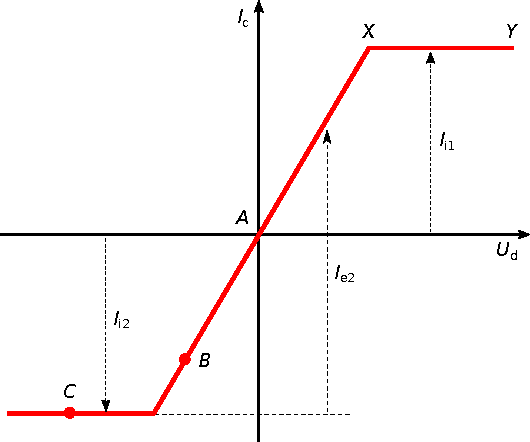
\includegraphics{vac-double}
	\caption{Voltampérová charakteristika dvojné sondy.
		Převzato z~\autocite{talsky}.}
	\label{fig:vac-double}
\end{figure}


\section{Jednoduchá sonda}
\label{sec:simple}
První sada pokusů byla provedena na aparatuře s~jednoduchou sondou
připojenou ke~zdroji stejnosměrného napětí.

\subsection{Metoda}
\label{sec:method-simple}
Schéma měřicí aparatury je na obrázku č.~\ref{fig:diagram-simple}.
Elektrody ve válcové výbojové trubici jsou připojeny k~laditelnému zdroji
stejnostměrného napětí a výbojový proud $\idisch$ je snímán ampérmetrem.
Válcová sonda o~poloměru $r=\SI{0.1}{\milli\metre}$
a délce $l=\SI{8}{\milli\metre}$ je umístěna poblíž anody.
Sondový obvod je napájen stejnosměrným zdrojem s~automatizovaým laděním.
Potenciál sondy $\potprobe$ a~sondový proud $\iprobe$ jsou měřeny
voltmetrem a~přesným ampérmetrem připojeným k~počítači.

\begin{figure}[htp]
	\centering
	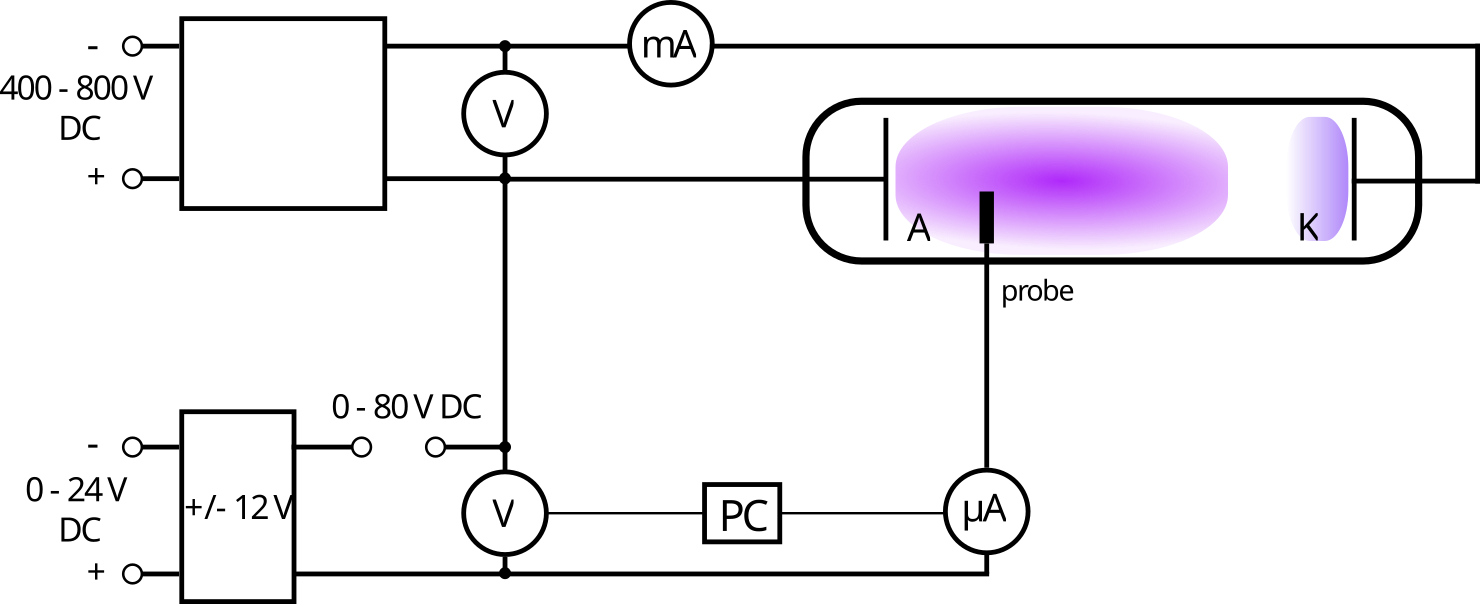
\includegraphics{diagram-simple.png}
	\caption{Uspořádání experimentu pro jednoduchou sondu.
		Převzato z~\autocite{assignment-simpleprobe}.}
	\label{fig:diagram-simple}
\end{figure}

Pro každou sadu podmínek byl nejprve přibližně určen plovoucí potenciál sondy
$\flpot$ jako bod, v~němž je proud sondou $\iprobe$ nulový.
Voltampérová charakteristika byla následně naměřena v~rozsahu~\SI{20}{\volt}
kolem plovoucího potenciálu.
Potenciál sondy byl automaticky lineárně zvyšován z~nejnižší hodnoty
na~nejvyšší a~zpět, čímž byly získány dvě datové sady.
Z~datových sad byly vyřazeny ty, u~nichž došlo k~nevysvětlenému kolísání
sondového proudu.
Kde zůstaly obě sady pro stejné podmínky, byly získány dvě voltampérové
charakteristiky, které byly zprůměrovány,

Hodnoty $\potprobe$ a~$\iprobe$ byly asynchronně zaznamenávány počítačem
spolu s~časovými značkami, které umožnily přiřazení odpovídajících hodnot
napětí a~proudu.
Vzhledem k~zaokrouhlení časových údajů na celé sekundy lze očekávat
nepřesnost přiřazení dat v~řádu desetin sekundy.

\subsubsection{Elektronový proud}
Levá část získané voltampérové charakteristiky byla proložena lineární funkcí
a~extrapolována pro celou oblast, kde nabývala záporných hodnot
(což nastalo pro všechny hodnoty potenciálu $\potprobe$).
Tato funkce byla považována za iontovou část sondového proudu $\iion$.
Elektronový proud byl získán odečtením iontového proudu od celkového:
\begin{equation}
	\label{eq:ielec}
	\ielec = \iprobe - \iion.
\end{equation}

\subsubsection{Plazmový potenciál}
\label{sec:plpot}
Potenciál neporušeného plazmatu $\plpot$ byl určen dvěma metodami.
První z~nich bylo stanovení tohoto potenciálu jako průsečíku přímek
proložených střední a~koncovou částí elektronového proudu v~logaritmickém
měřítku.
Tento způsob je zde nazýván metodou asymptot.

Druhá metoda vychází z~poznatku, že v~okolí plazmového potenciálu $\plpot$
bude mít voltampérová charakteristika inflexní bod:
Elektronový proud byl kvůli potlačení šumu vyhlazen polynomem osmého stupně
a plazmový potenciál byl stanoven jako nulový bod druhé derivace $\didu$
proloženého polynomu.

\subsubsection{Elektronová teplota}
Ze směrnice přímky proložené střední částí charakteristiky byla určena
elektronová teplota $\tempelec$ podle vztahu:
\begin{equation}
	\label{eq:tempeleca}
	\tempeleca = \frac{\elemcharge}{\boltzmann \slopeb},
\end{equation}
kde $\slopeb$ je směrnice proložené přímky.
%
Pro porovnání byla elektronová teplota určena také z~plovoucího potenciálu
$\flpot$ jako:
\begin{equation}
	\label{eq:tempelecp}
	\tempelecp = \frac{2\elemcharge}{\boltzmann}
		\ln\left(\frac{4\pi\masselec}{\massion}\right)
		|\flpot - \plpot|,
\end{equation}
kde $\massion$ je hmotnost iontu pracovního plynu, kterým byl argon,
proto $\massion = \SI{40}{\atomicmassunit} = \SI{6.6422e-26}{\kilogram}$.

\subsection{Výsledky}
\label{results-simple}
Naměřené voltampérové charakteristiky jsou na obrázcích
č.~\ref{fig:simple1-vac-1}--\ref{fig:simple1-vac-2}.
Spočtené hodnoty plovoucího a~plaz\-mo\-vého potenciálu a~elektronové teploty
jsou v~souhrnné tabulce č.~\ref{tab:comparison}.
Pozoruhodné je, že plazmové potenciály určené oběma metodami vycházejí
(až na případ vysokého tlaku $\pres$) vůči sobě posunuty o~zhruba konstatní
hodnotu:
Potenciál z~metody asymptot je vždy asi o~$\SI{3}{\volt}$ nižší.
Tento jev se nepodařilo objasnit.

\begin{figure}[p]
	\centering
	\input{plots/simple1-vac-1}
	\input{plots/simple1-vac-log-1}
	\par\smallskip
	\input{plots/simple1-vac-2}
	\input{plots/simple1-vac-log-2}
	\par\smallskip
	\input{plots/simple1-vac-3}
	\input{plots/simple1-vac-log-3}
	\par\smallskip
	\input{plots/simple1-vac-4}
	\input{plots/simple1-vac-log-4}
	\caption{Voltampérové charakteristiky jednoduché sondy
		v~jednoduchém zapojení (1.~část).
		$\idisch$ je výbojový proud a~$\pres$ je tlak.
		Plazmové potenciály jsou $\plpotd$ (určený z~druhé derivace)
		a~$\plpota$ (určený z~metody asymptot).}
	\label{fig:simple1-vac-1}
\end{figure}
\begin{figure}[p]
	\centering
	\input{plots/simple1-vac-5}
	\input{plots/simple1-vac-log-5}
	\par\smallskip
	\input{plots/simple1-vac-6}
	\input{plots/simple1-vac-log-6}
	\par\smallskip
	\input{plots/simple1-vac-7}
	\input{plots/simple1-vac-log-7}
	\caption{Voltampérové charakteristiky jednoduché sondy
		v~jednoduchém zapojení (2.~část).
		$\idisch$ je výbojový proud a~$\pres$ je tlak.
		Plazmové potenciály jsou $\plpotd$ (určený z~druhé derivace)
		a~$\plpota$ (určený z~metody asymptot).}
	\label{fig:simple1-vac-2}
\end{figure}


\clearpage
\section{Jednoduchá sonda s~oscilujícím napětím}
\label{sec:eedf}
Druhá sada pokusů byla provedena na téže aparatuře s~modifikací,
která umožňovala k~napětí sondy přidat malé střídavé napětí.
Zpracování bylo podobné jako v~předchozí části,
byla však navíc vyhodnocena rozdělovací funkce elektronů podle energie.

\subsection{Metoda}
\label{sec:method-eedf}
Aparatura popsaná v~části \ref{sec:method-simple} je upravena
vložením transformátoru do~sondového obvodu,
jak je znázorněno na~obrázku č.~\ref{fig:diagram-eedf}.
Vnější obvod transformátoru je napájen střídavým napětím,
ve vnitřním obvodu je indukováno malé střídavé napětí,
které se sčítá s~větším stejnosměrným napětím ze zdroje.

\begin{figure}[hbp]
	\centering
	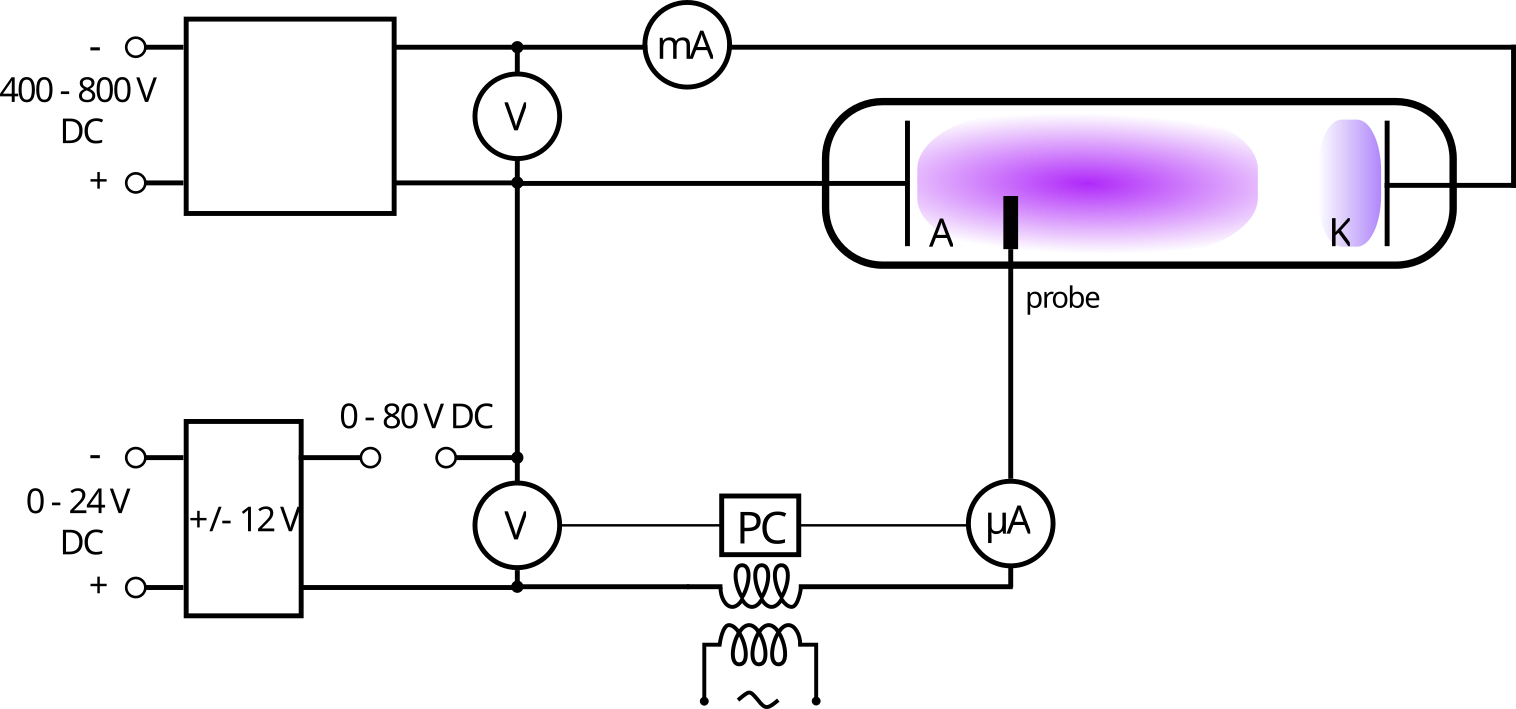
\includegraphics{diagram-eedf.png}
	\caption{Uspořádání experimentu pro jednoduchou sondu se střídavým napětím.
		Převzato z~\autocite{assignment-simpleprobe}.}
	\label{fig:diagram-eedf}
\end{figure}

\subsubsection{Rozdělovací funkce elektronů}
\label{sec:eedf-eedf}
Rozdělovací funkce elektronů podle energie $\eedf$ byla určena ze vztahu:
\begin{equation}
	\label{eq:eedf}
	\eedf = \frac{1}{\probesurf}
		\sqrt{\frac{8\,\masselec}{\elemcharge^3}\,|\uprobe|}
		\,\frac{\mathrm d^2 \ielec}{\mathrm d\uprobe^2},
\end{equation}
kde $\probesurf$ je plocha sondy, $\masselec$ je hmotnost elektronu
a $\elemcharge$ elementární náboj.
Derivace voltampérové charakteristiky $\didu$ byla stanovena dvěma způsoby,
což vedlo ke~dvěma variantám rozdělovací funkce.

Prvním způsobem byla numerická derivace naměřených dat po vyhlazení.
Toto bylo provedeno na voltampérové charakteristice získané bez~střídavého
napětí, vyhlazení bylo provedeno polynomem osmého stupně,
stejně jako při určování plazmového potenciálu v~části \ref{sec:plpot}.

Druhým přístupem je využití střídavého napětí, které aparatura umožňuje.
Předpokládejme, že ke stejnosměrnému napětí sondy je přidána malá
střídavá složka $\ueedf\cdot\sin{\omega t}$,
jejíž amplituda je výrazně menší než stejnosměrné napětí.
V~takovém případě dojde k~nárůstu sondového proudu o~hodnotu,
již lze v~prvním přiblížení vyjádřit následovně:
\begin{equation}
	\label{eq:eedf-idiff}
	\Delta\iprobe \approx \frac{\ueedf^2}{4}\didu.
\end{equation}
Změřením charakteristiky se~střídavým napětím i~bez něj lze přírůstek
$\Delta\iprobe$ přímo určit.

\subsubsection{Charakterizace rozdělovací funkce}
Získané rozdělovací funkce byly aproximovány variantami následujícího
rozdělení pomocí metody nejmenších čtverců:
\begin{equation}
	\label{eq:model}
	\eedf = a \sqrt{\enelec}
		e^{(\frac{-\enelec}{\boltzmann\tempelec})^\kappa}.
\end{equation}
Aproximované parametry vždy zahrnovaly parametr $a$ a~teplotu $\tempelec$.
V~první variantě bylo $\kappa = 1$, což odpovídá Maxwellovu-Boltzmannovu
rozdělení.
V~druhé bylo $\kappa = 2$, takové rozdělení se nazývá Druy\-ve\-steynovo.
Třetí variantou bylo rozdělení s~obecným exponentem $\kappa$,
který se stal třetím hledaným parametrem.

\subsubsection{Měřicí procedura}
Aby bylo možno měřit sondový proud zároveň se~střídavým napětím i~bez něj,
bylo nutno přizpůsobit průběh experimentu.
Měření probíhalo souvisle a~střídavý proud byl v~pětisekundových intervalech
zapínán a~vypínán.
Tím vznikla jedna datová řada, kterou bylo třeba rozdělit.
To bylo provedeno spočtením klouzavého průměru oknem o~délce třiceti bodů,
který sloužil jako rozhodovací funkce.
Body nad~rozhodovací funkcí byly přisouzeny stavu se~zapnutým střídavým
napětím, body pod~ní stavu bez~střídavého napětí.
Oba získané průběhy byly posléze proloženy polynomem osmého stupně,
aby se překrývaly.
Příklad tohoto postupu je na~obrázku č.~\ref{fig:separation}.

Vyhodnocení dat bylo prováděno na sadě bez~střídavého napětí,
data se~střídavým napětím posloužila pouze pro získání přírůstku
sondového proudu $\Delta\iprobe$.

\begin{figure}[hbp]
	\centering
	\input{plots/separation}
	\caption{Příklad rozdělení dat do sérií se~střídavým napětím a bez~něj.
		Čárkovaná rozhodovací funkce je klouzavý průměr z~třiceti bodů.}
	\label{fig:separation}
\end{figure}

\subsection{Výsledky}
\label{sec:results-eedf}
Měření bylo provedeno pro tři kombinace tlaku $\pres$ a~výbojového
proudu $\idisch$.
Na obrázku č.~\ref{fig:simple2-vac} je uvedeno zpracování v~rozsahu
analogickém části~\ref{sec:simple}.
Rozdělovací funkce $\eedf$ určené podle obou variant derivace $\didu$
jsou na obrázku č.~\ref{fig:eedf} spolu s~optimalizovanými modelovými
funkcemi a~jejich parametry.

\begin{figure}[p]
	\centering
	\input{plots/simple2-vac-1}
	\input{plots/simple2-vac-log-1}
	\par\smallskip
	\input{plots/simple2-vac-2}
	\input{plots/simple2-vac-log-2}
	\par\smallskip
	\input{plots/simple2-vac-3}
	\input{plots/simple2-vac-log-3}
	\caption{Voltampérové charakteristiky jednoduché sondy
		v~zapojení s~oscilujícím napětím
		pro měření rozdělovací funkce elektronů.
		$\idisch$ je výbojový proud a~$\pres$ je tlak.
		Plazmové potenciály jsou $\plpotd$ (určený z~druhé derivace)
		a~$\plpota$ (určený z~metody asymptot).}
	\label{fig:simple2-vac}
\end{figure}

\begin{figure}[p]
	\centering
	\input{plots/simple2-eedf-1}
	\par\smallskip
	\input{plots/simple2-eedf-2}
	\par\smallskip
	\input{plots/simple2-eedf-3}
	\caption{Normované rozdělovací funkce elektronů $\eedf$ podle energie určené
		oběma metodami: z~numerické derivace proloženého polynomu (červené)
		a~z~derivace změřené pomocí střídavého napětí (modré).
		Průběhy jsou aproximovány teoretickými rozděleními s~různými hodnotami
		exponentu $\kappa$:
		Max\-wellovým-Boltzmannovým ($\kappa = 1$),
		Druyvesteynovým ($\kappa = 2$)
		a~rozdělením s~obecným $\kappa$.}
	\label{fig:eedf}
\end{figure}


\clearpage
\section{Dvojná sonda}
\label{sec:double}
% \renewcommand\iion{I_\mathrm{i}}
Třetí sada pokusů se zabývala dvojnou sondou.
Zkoumanými veličinami byly především elektronová teplota a~hustota.

\subsection{Metoda}
\label{sec:method-double}
Schéma aparatury je na~obrázku č.~\ref{fig:diagram-double}.
Záznam napětí a~proudu je automatizován stejným způsobem jako
v~předchozích částech.

\begin{figure}[hbp]
	\centering
	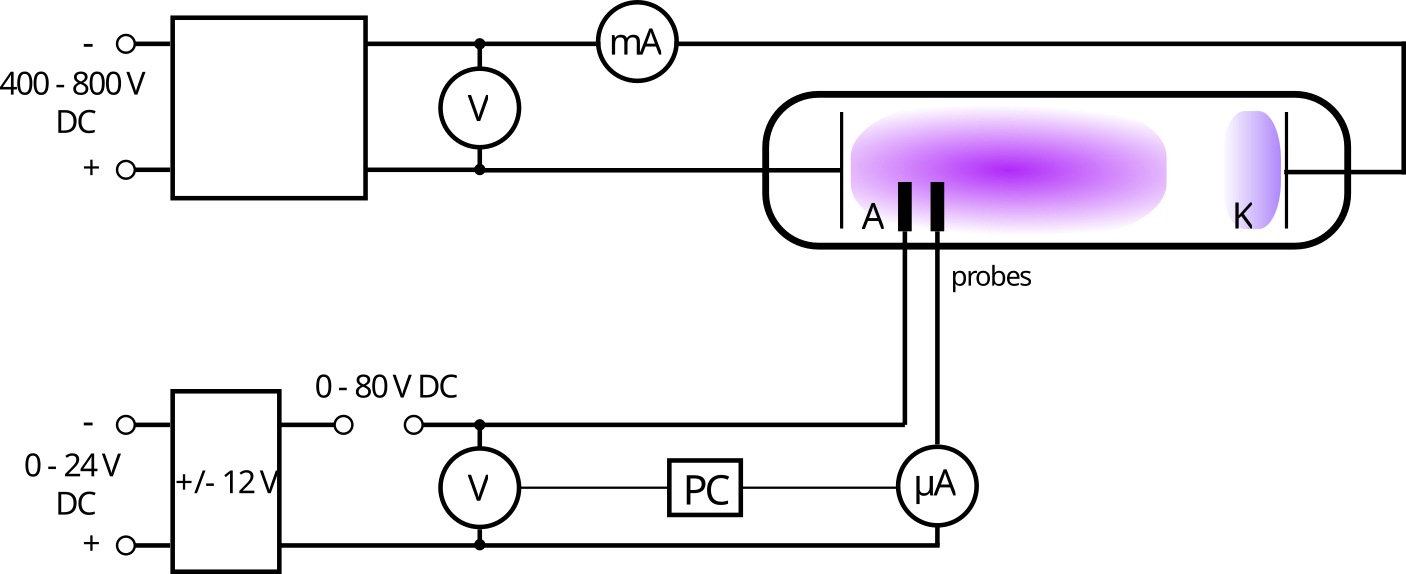
\includegraphics{diagram-double.png}
	\caption{Uspořádání experimentu s~dvojnou sondou.
		Převzato z~\autocite{assignment-doubleprobe}.}
	\label{fig:diagram-double}
\end{figure}

\subsubsection{Iontový a~elektronový proud}
Iontové proudy $\iioni$ a~$\iionii$ pro nulové napětí na sondě $\udouble$
byly určeny průsečíkovou metodou z~celkového proudu.
Proudy ve střední části a v~obou větvích byly proloženy přímkami.
Průsečík přímky nasyceného proudu v~příslušné větvi s~přímkou proloženou
střední částí byl pomocný bod~X.
Iontový proud byl odečten z~přímky nasyceného proudu v~jedné pětině
úsečky vedoucí od osy~$\idouble$ k~bodu~X.

Elektronové proudy byly určeny jako rozdíl příslušného iontového proudu
a~celkového proudu při nulovém napětí na~sondě:
\begin{align}
	\label{eq:ieleci}
	\ieleci  &= \iioni  - \idouble(\udouble = 0) \\
	\ielecii &= \iionii - \idouble(\udouble = 0)
\end{align}

\subsubsection{Elektronová teplota}
\label{sec:double-tempelec}
Elektronová teplota byla určena dvěma metodami.
V~první metodě byl nejprve stanoven takzvaný ekvivalentní odpor
dvojné sondy~$\eqresist$ jako směrnice přímky proložené střední
částí charakteristiky.
Teplota pak byla spočtena podle vztahu:
\begin{equation}
	\label{eq:tempeleca-double}
	\tempeleca = \frac{\elemcharge}{\boltzmann}
		(G - G^2) \eqresist \sum \iion,
\end{equation}
kde veličina $G$ je poměr proudů:
\begin{equation}
	\label{eq:g}
	\frac{\ielecii}{\sum \iion}.
\end{equation}

\newcommand\paramc{\alpha}
\newcommand\parame{\beta}
V~druhé variantě byla charakteristika proložena následující zobecněnou
charakteristikou (srovnej ideální charakteristiku \eqref{eq:double-ideal})
a~teplota určena z~nalezeného parametru:
\begin{equation}
	\label{eq:double-fit}
	\idouble = \iionsat\,
		\tgh\left(
			\frac{\elemcharge\udouble}{\boltzmann\tempelec} + \paramc
		\right)
		+ \parame.
\end{equation}

\subsubsection{Elektronová hustota}
Koncentrace elektronů byla stanovena nepřímo z~koncentrace iontů
pomocí předpokladu, že v~kvazineutrálním plazmatu bez vícenásobné ionizace
se tyto hustoty musejí rovnat.
Iontová hustota byla určena z~iontového proudu pomocí vztahu:
\begin{align}
	\label{eq:denselec-iion}
	\denselec &\approx \dension = \frac{4 \iion}
		{\sheathsurf \, \denselec \, \langle\speedion\rangle} &
	\langle\speedion\rangle &= \sqrt\frac{8 \boltzmann \tempion}{\pi\massion},
\end{align}
kde $\langle\speedion\rangle$ je střední rychlost iontů
a~$\sheathsurf$ je plocha stěnové vrstvy sondy
odhadnutá na~$\SI{5}{\centi\meter\squared}$.
Iontový proud na jednu sondu $\iion$ byl spočten jako průměr proudů
$\iioni$ a~$\iionii$.
Teplota iontů $\tempion$ nebyla známa, zde byla nahrazena teplotou elektronů.

Pro porovnání byla teplota také spočtena z~nasyceného iontového proudu
ze vztahu:
\begin{equation}
	\label{eq:denselec-iionsat}
	\iionsat = \num{0.61} \denselec\sheathsurf
		\sqrt\frac{\boltzmann\tempelec}{\massion},
\end{equation}
kde nasycený proud $\iionsat$ byl určen z~parametrů proložené
funkce~\eqref{eq:double-fit}.

\subsection{Výsledky}
\label{sec:results-double}

\begin{figure}
	\centering
	\input{plots/double-vac-1}
	\input{plots/double-vac-2}
	\par\smallskip
	\input{plots/double-vac-3}
	\input{plots/double-vac-4}
	\caption{Voltampérové charakteristiky dvojné sondy
		a~zpracování pomocí průsečíkové metody.
		Zde $\idisch$ je výbojový proud a~$\pres$ je tlak.}
	\label{fig:double-vac}
\end{figure}

\begin{figure}
	\centering
	\input{plots/double-fit}
	\caption{Aproximace voltampérových charakteristik dvojné sondy
		pro uvedené hodnoty výbojového proudu $\idisch$ a~tlaku $\pres$.
		Naměřená data jsou pro přehlednost decimována.}
	\label{fig:double-fit}
\end{figure}

\section{Porovnání}
\label{sec:comparison}

\shorthandoff{-}
\begin{table}[bh]
	\centering
	\caption{Porovnání výsledků různých metod.
		Plazmový potenciál $\plpota$ byl určen metodou asymptot,
		$\plpotd$ z~druhé derivace elektronového proudu.
		Elektronová teplota $\tempeleca$ byla určena z~metody asymptot,
		$\tempelecp$ z~plovoucího potenciálu
		a~$\tempelecf$ z~aproximace rozdělovací funkce obecným rozdělením.
		Exponent $\kappa$ je parametr tohoto rozdělení.
	}
	\label{tab:comparison}
	\newcommand\rowsep{\medskip}
	\sisetup{
		table-alignment-mode = format,
		table-number-alignment = center,
	}
	\pgfplotstabletypeset[
		header = false,
		col sep = tab,
		skip first n = 1,
		every head row/.style = {
			before row = \toprule,
			after row = {
				\midrule
				\multicolumn{6}{l}{\small\bf{jednoduchá sonda}} \\
			}
		},
		string type,
		columns = {[index] 0, [index] 1, [index] 2, [index] 3, [index] 4,
			[index] 5, [index] 6, [index] 7, [index] 8},
		columns/0/.style = {
			column name = $\pres\ [\si{\pascal}]$,
			column type = {S[table-format = 3.0]},
		},
		columns/1/.style = {
			column name = $\idisch\ [\si{\milli\ampere}]$,
			column type = {S[table-format = 2.0]},
		},
		columns/2/.style = {
			column name = $\flpot\ [\si{\volt}]$,
			column type = {S[
				table-format = -2.1,
				round-mode = places,
				round-precision = 1
			]},
		},
		columns/3/.style = {
			column name = $\plpota\ [\si{\volt}]$,
			column type = {S[
				table-format = -2.1,
				round-mode = places,
				round-precision = 1
			]},
		},
		columns/4/.style = {
			column name = $\plpotd\ [\si{\volt}]$,
			column type = {S[
				table-format = -2.1,
				round-mode = places,
				round-precision = 1
			]},
		},
		columns/5/.style = {
			column name = $\tempeleca\ [\si{\kelvin}]$,
			column type = {S[
				table-format = 5.0,
				round-mode = figures,
				round-precision = 3
			]},
		},
		columns/6/.style = {
			column name = $\tempelecp\ [\si{\kelvin}]$,
			column type = {S[
				table-format = 5.0,
				round-mode = figures,
				round-precision = 3
			]},
		},
		columns/7/.style = {
			column name = $\tempelecf\ [\si{\kelvin}]$,
			column type = {S[
				table-format = 5.0,
				round-mode = figures,
				round-precision = 3
			]},
			string replace={0}{},
		},
		columns/8/.style = {
			column name = $\kappa$,
			column type = {S[
				table-format = 1.2,
				round-mode = places,
				round-precision = 2
			]},
			string replace={0}{},
		},
		every row no 6/.style = {before row = \medskip},
		every row no 7/.style = {before row = {
			\multicolumn{6}{l}{\small\bf{jednoduchá sonda se~střídavým napětím}} \\
		}},
		every last row/.style = {after row = \bottomrule}
	]{results/comparison.tsv}
\end{table}
\shorthandon{-}

\shorthandoff{-}
\begin{table}[bh]
	\centering
	\caption{Výsledky experimentu s~dvojnou sondou.}
	\label{tab:comparison-double}
	\sisetup{
		table-alignment-mode = format,
		table-number-alignment = center,
	}
	\pgfplotstabletypeset[
		outfile = results/comparison-double.tex,
		header = false,
		col sep = tab,
		skip first n = 1,
		every head row/.style = {
			before row = \toprule,
			after row = {
				\midrule
			}
		},
		string type,
		columns = {[index] 0, [index] 1, [index] 2, [index] 3, [index] 4,
			[index] 5, [index] 6},
		columns/0/.style = {
			column name = $\pres\ [\si{\pascal}]$,
			column type = {S[table-format = 3.0]},
		},
		columns/1/.style = {
			column name = $\idisch\ [\si{\milli\ampere}]$,
			column type = {S[table-format = 2.2]},
		},
		columns/2/.style = {
			column name = $\tempeleca\ [\si{\kelvin}]$,
			column type = {S[
				table-format = 5.0,
				round-mode = figures,
				round-precision = 3
			]},
		},
		columns/3/.style = {
			column name = $\tempelecf\ [\si{\kelvin}]$,
			column type = {S[
				table-format = 5.0,
				round-mode = figures,
				round-precision = 3
			]},
		},
		columns/4/.style = {
			column name = $\denseleca\ [\si{\per\metre\cubed}]$,
			column type = {S[
				table-format = 1.3e2,
				round-mode = places,
				round-precision = 3,
				exponent-mode = scientific
			]},
		},
		columns/5/.style = {
			column name = $\denselecf\ [\si{\per\metre\cubed}]$,
			column type = {S[
				table-format = 1.3e2,
				round-mode = places,
				round-precision = 3,
				exponent-mode = scientific
			]},
		},
		columns/6/.style = {
			column name = $\denselecfii\ [\si{\per\metre\cubed}]$,
			column type = {S[
				table-format = 1.3e2,
				round-mode = places,
				round-precision = 3,
				exponent-mode = scientific
			]},
		},
		every last row/.style = {after row = \bottomrule}
	]{results/comparison-double.tsv}
\end{table}
\shorthandon{-}

\printbibliography
\end{document}
